\documentclass{article}
\usepackage[utf8]{inputenc}
\usepackage{mathtools,amssymb}
\usepackage{lipsum}
\usepackage{hyperref}
\usepackage{layout}
\usepackage{geometry}
\usepackage{listings}
\usepackage{booktabs}       % professional-quality tables
\usepackage{color}
\usepackage{pdfpages}
\usepackage{algorithm}
\usepackage{algpseudocode}
\usepackage{graphicx}
\graphicspath{{"../results/"}}
\newcommand*{\vertbar}[1][10ex]{\rule[-1ex]{0.5pt}{#1}}
\newcommand*{\horzbar}{\rule[.5ex]{2.5ex}{0.5pt}}
\newcommand{\norm}[2]{\left\lVert#1\right\rVert_#2}
\newcommand{\abs}[1]{\lvert#1\rvert}

\title{STATS370: Final Project}
\author{Erich Trieschman}
\date{2022 Fall Quarter}


\newcommand{\userMarginInMm}{10}
\geometry{
 left=12 mm,
 right=12 mm,
 top=20 mm,
 bottom=20 mm,
 footskip=5mm}

\newcommand*\circled[1]{\raisebox{.5pt}{\textcircled{\raisebox{-.9pt} {#1}}}}
\newcommand*\bspace{$\; \bullet \;$}

\hypersetup{
    colorlinks=true,
    linkcolor=blue,
    filecolor=magenta,      
    urlcolor=cyan,
    pdfpagemode=FullScreen,
}

\definecolor{dkgreen}{rgb}{0,0.6,0}
\definecolor{gray}{rgb}{0.5,0.5,0.5}
\definecolor{mauve}{rgb}{0.58,0,0.82}
    
\lstset{frame=tb, language=Python,
  aboveskip=3mm,
  belowskip=3mm,
  showstringspaces=false,
  columns=flexible,
  basicstyle={\small\ttfamily},
  numbers=none,
  numberstyle=\tiny\color{gray},
  keywordstyle=\color{blue},
  commentstyle=\color{dkgreen},
  stringstyle=\color{mauve},
  breaklines=true,
  breakatwhitespace=true,
  tabsize=3}

\begin{document}
\maketitle

% \tableofcontents

\section*{Introduction}
\begin{itemize}
  \item Compute quantiles, plot histograms, obtain means, variances and correlation matrix.
  \item Check convergence of the chain: does the variance of the distribution stabilize? Run two markov chains, how do they compare?
  \item Hamiltonian: Parameter search. Implement over M, eps, L. See section 3.5 for tuning
  \item Gibbs: basically show the math
  \item Metropolis Hasting: choice of candidate distribution. Make sure domain is right for each, could optimize parameters of the candidate distributions
  \item Importance sampling: TBD
\end{itemize}

%------------------------------------------------------------------------
% METROPOLIS HASTINGS
\section{Metropolis Hasting}
\label{sec:MH}
\subsection{Implementation}
In this section I use the Methropolis-Hasting algorithm to generate samples from my posterior distribution of model parameters. At each step, this algorithm requires the choice of a candidate distribution, $q(\theta)$, from which to draw candiate samples, and accepts those samples according to an acceptance probability that is determined by the currently selected sample. Under a sufficient sample size, the statistics generated from my sample approximate the true statistics of the target distribution, which allows me to study this distribution. 

I choose the candidate distribution at each step to match the support of the target parameter space. To facilitate implementation, I construct distributions with the same shape at each step, only shifted so that the mean of the candidate distribution is located at the current accepted sample point. In this way I can propose candidates with a higher likelihood of being accepted. To facilitate implementation, my candidate distribution is the composition of independent distributions for each parameter. In Algorithm \ref{alg:mh} I present my implemented approach.

\begin{algorithm}[h]
  \caption{\label{alg:mh}Metropolis Hastings algorithm}
    \begin{algorithmic}[1]
      \State $\theta_0 \longleftarrow$  Initialize
      \For{t=0, \dots, T}
        \State $\theta_{cand} \sim q(\theta) := q(\sigma^2\mid\sigma^2_t)q(\tau\mid\tau_t)q(\mu\mid\mu_t)q(\gamma \mid \gamma_t)$
        \State $a_t \longleftarrow \min\left(\frac{f(\theta_{cand})q(\theta_t\mid\theta_{cand})}{f(\theta_t)p(\theta_{cand}\mid\theta_t)}\right)$
        \State $u_t \sim Unif[0,1]$
        \If{$u_t \leq a_t$}
          \State $\theta_{t+1} \longleftarrow \theta_{cand}$
        \Else 
          \State $\theta_{t+1} \longleftarrow \theta_t$
        \EndIf
      \EndFor
    \end{algorithmic}
  \end{algorithm}


In Table \ref{tab:mh_cand} I describe the independent probability distributions used for my candidate distribution, assuming at step i that $\theta_i = (\sigma^2_i, \tau_i, \mu_i, \gamma_i)$.

\begin{table}[H]
  \small
  \begin{center}
    \begin{tabular}{lr}
    \textbf{Parameter} & \textbf{Distribution} \\
    \midrule
    $e^{\sigma^2_{i+1}}$ & $Norm(\mu=\log(\sigma^2_i), \sigma^2=\nu_{\sigma^2})$\\
    $\tau_{i+1}$ & $TruncNorm(\mu=\tau_i, \sigma^2=\nu_{\tau}, lb=0, ub=1)$\\
    $\mu_{i+1}$ & $Norm(\mu=\mu_i, \Sigma=\nu_{\mu}I)$\\
    $\gamma_{i+1}$ & $Norm(\mu=\gamma_i, \Sigma=\nu_{\gamma}I)$\\
    \bottomrule
    \end{tabular}
    \end{center}
    \caption{\label{tab:mh_cand} Form of candidate distribution, assuming independence across distributions}
\end{table}

Note that I transform $\sigma^2$ so that it can follow a log-normal distribution so my proposals lie in its domain. To properly implement this, I include the jacobian of the transformation, as shown below.

\begin{align}
  q(\theta \mid \theta_i) &=  q(\sigma^2\mid\sigma^2_i) q(\tau\mid\tau_i)q(\mu\mid\mu_i)q(\gamma \mid \gamma_i), \textrm{ where }\\
  q(\sigma^2 \mid \sigma^2_i) &= \frac{1}{\sqrt{2\pi\nu_{\sigma^2}}}\exp\left[\frac{1}{2\nu_{\sigma^2}}\left(\log(\sigma^2) - \log(\sigma^2_i)\right)^2\right]\left| \frac{d}{d\sigma^2}\log(\sigma^2)\right|  
\end{align}

In this algorithm I have ample flexibility to define my candidate distribution, $q(\theta)$. To tune this algorithm, my objective is to construct a candidate distribution that proposes candidates with high probability of being accepted. After all, the higher the acceptance rate, the more samples I can generate per iteration of the algorithm. 

Yet, naively constructing an effective candidate distribution can be difficult as such a distribution needs to propose samples that i) sufficiently explore the entire parameter space and ii) have a high enough probability of returning to the original sample. In my implementation of this algorithm, I notice a tradeoff between these requirements, where lower-variance distributions around the current sample points increase the acceptance probability, but also increase the autocorrelation between points. Reducing autocorrelation between sample points in important to reduce bias of the overall sample. I use a grid search to optimize this tradeoff by tuning the variance in each distribution above, $(\nu_{\sigma^2}, \nu_\tau, \nu_\mu, \nu_\gamma)$, noting in the literature that an optimal acceptance rate for this tradeoff is between 0.25 and 0.35 when the parameter space is greater than 4 dimensions \cite{Roberts}. Table \ref{tab:mh_gridsearch} in Appendix \ref{sec:a_mh} details the results of my tuning. 

\subsection{Results}
Below I present results from running the Metropolis-Hastings algorithm for $T=100,000$ iterations. Figure \ref{fig:mh_dist} and Figure \ref{fig:mh_acorr} visualize the acceptance rate of each candidate sample point and the autocorrelation, the two the performance metrics used for the grid search above, and Figure \ref{fig:mh_marg} visualizes the sample points drawn from this algorithm at each step (left side), as well as their accumulated marginal distributions (right side).

\begin{figure}[H]
  \centering
  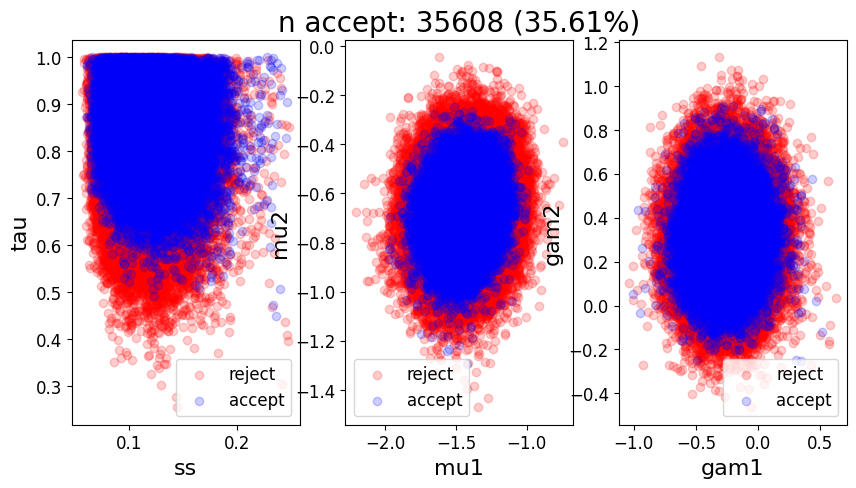
\includegraphics[width=.8\linewidth]{"./mh_dist.png"}
  \caption{\label{fig:mh_dist} Bivariate distributions for accepted and rejected candidate parameters drawn from Metropolis-Hastings}
\end{figure}

\begin{figure}[H]
  \centering
  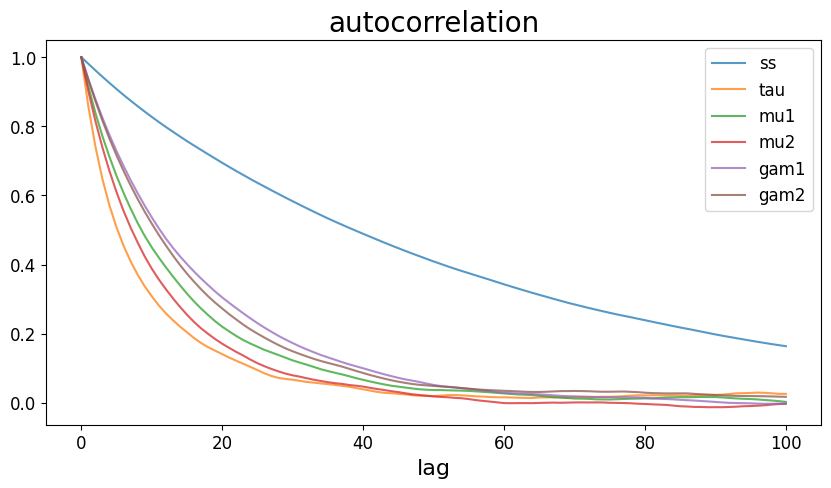
\includegraphics[width=.8\linewidth]{"./mh_acorr.png"}
  \caption{\label{fig:mh_acorr} Autocorrelation for each parameter drawn from Metropolis-Hastings}
\end{figure}

\begin{figure}[H]
  \centering
  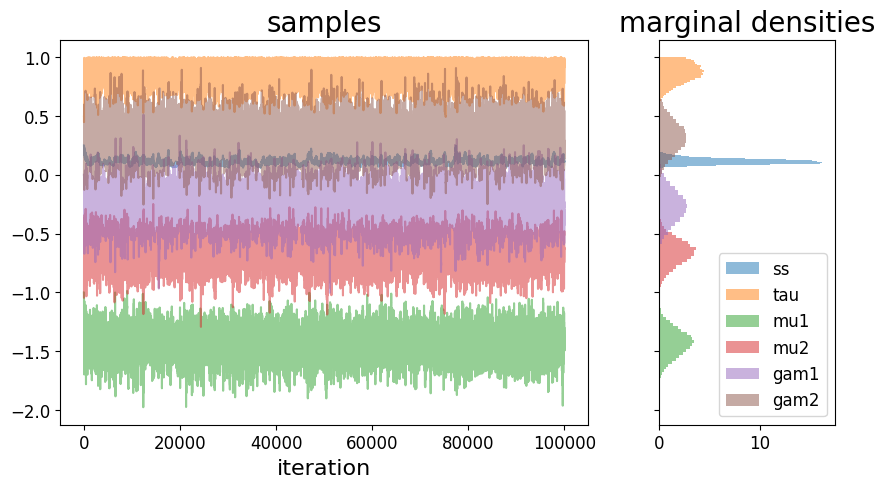
\includegraphics[width=.8\linewidth]{"./mh_marg.png"}
  \caption{\label{fig:mh_marg} Evolution of the Metropolis-Hastings sampling algorithm and accumulated marginal distributions}
\end{figure}

Next I present univariate statistics in Table \ref{tab:mh_univar} as well as the covariance between each parameter pair in Table \ref{tab:mh_covar}. 

\begin{table}[H]
  \begin{center}
    \begin{tabular}{lrrrrrr}
      {} &$\sigma^2$ & $\tau$ & $\mu_1$ & $\mu_2$ & $\gamma_1$ & $\gamma_2$ \\
      \midrule
      mean   &  0.128855 &  0.856592 & -1.437832 & -0.660407 & -0.269792 &  0.316120 \\
      var    &  0.000854 &  0.007508 &  0.016422 &  0.013851 &  0.024934 &  0.023575 \\
      median &  0.124435 &  0.864481 & -1.432695 & -0.657491 & -0.270956 &  0.317396 \\
      p0     &  0.060584 &  0.389299 & -2.154638 & -1.326388 & -0.958255 & -0.361611 \\
      p10    &  0.095844 &  0.738386 & -1.602141 & -0.809834 & -0.470537 &  0.121178 \\
      p25    &  0.107768 &  0.798937 & -1.520030 & -0.735483 & -0.373689 &  0.214412 \\
      p50    &  0.124435 &  0.864481 & -1.432695 & -0.657491 & -0.270956 &  0.317396 \\
      p75    &  0.145736 &  0.924773 & -1.350404 & -0.580824 & -0.166230 &  0.418696 \\
      p90    &  0.167346 &  0.966222 & -1.279685 & -0.514553 & -0.070925 &  0.509682 \\
      p100   &  0.327578 &  0.999997 & -0.861472 & -0.172091 &  0.399618 &  0.980294 \\
      \bottomrule
      \end{tabular}
  \end{center}
  \caption{\label{tab:mh_univar} Univariate statistics from samples drawn from Metropolis-Hastings}
\end{table}

\begin{table}[H]
  \begin{center}
    \begin{tabular}{lrrrrrr}
      {} & $\sigma^2$ & $\tau$ & $\mu_1$ & $\mu_2$ & $\gamma_1$ & $\gamma_2$ \\
      \midrule
      $\sigma^2$   &  0.000854 & -0.000323 & -0.000197 & -0.000117 &  0.000087 & -0.000238 \\
      $\tau$  & -0.000323 &  0.007508 &  0.005160 &  0.003291 & -0.000687 &  0.000761 \\
      $\mu_1$  & -0.000197 &  0.005160 &  0.016422 &  0.002575 & -0.007119 &  0.000374 \\
      $\mu_2$  & -0.000117 &  0.003291 &  0.002575 &  0.013851 & -0.000793 & -0.005262 \\
      $\gamma_1$ &  0.000087 & -0.000687 & -0.007119 & -0.000793 &  0.024934 & -0.000133 \\
      $\gamma_2$ & -0.000238 &  0.000761 &  0.000374 & -0.005262 & -0.000133 &  0.023575 \\
      \bottomrule
      \end{tabular}
  \end{center}
  \caption{\label{tab:mh_covar} Covariance between parameters from distributions drawn from Metropolis Hastings}
\end{table}


% =================================== TODO ====================================
In these tables I observe PLACEHOLDER




% -------------------------------------------------------------------------------
% GIBBS
\section{Gibbs sampling}
\subsection{Implementation}
In this section I use the Gibbs sampling algorithm to generate samples from my posterior distribution of model parameters. Much like the Metropolis-Hastings algorithm, this approach generates candidate samples from a candidate distribution leveraging the properties of Markov Chains. 

Gibbs sampling is a strict improvement over the naive Metropolis-Hastings algorithm because the algorithm proposes candidates that are accepted at every step. A second advantage of this result is that the proposal candidates also explore the parameter space with very little autocorrelation because the jump probabilities are always sufficiently high. Therefore, Gibbs sampling is capable of maximizing both of the criteria (acceptance probability and autocorrelation) that I seek to tune in my naive Metropolis Hastings algorithm. As we prove in lecture, this success is accomplished because the candidate distributions are simply the target distribution of each parameter, conditional on the values of each other parameter. 

\begin{align}
  p(\theta[i] \mid Y, \theta[-i]) = \frac{p(\theta[i], \theta[-i] \mid Y)}{p(\theta[-i] | Y)} = f(\theta[i]) \propto p(\theta \mid Y) \textrm{ with fixed } \theta[-i], Y
\end{align}

The challenge presented by Gibbs sampling is the need for a closed form probability distribution for each conditional target distribution. Fortunately, in this project I was able to derive these distributions; my work is included in Appendix \ref{sec:a_gibbs}. In the general case, however, such closed form distributions may not exist.

While the Gibbs sampling algorithm does not require hyperparameter tuning, it does require that I determine order in which to scan and update the candidate parameter values. The two most common approaches are i) a systematic scan of the variables in the same order in each algorithm step and ii) a random scan of the variables (without replacement) in each algorithm step. I choose the latter approach, although I note that both approaches yield very similar results. 

I present my implemented Gibbs sampling approach in Algorithm \ref{alg:gibbs}. 
\begin{algorithm}[H]
  \caption{\label{alg:gibbs}Gibbs sampling algorithm}
    \begin{algorithmic}[1]
      \State $\theta_0 \longleftarrow$  Initialize
      \For{t=0, \dots, T}
        \State $idx \longleftarrow$ Shuffle($0,1,2,3,4,5$) \Comment{Randomize index order}
        \State $\theta_{cand} \longrightarrow \theta_t$
        \For{i in {$idx$}}
          \State $\theta_{cand}[i] \sim p(\theta[i] \mid Y, \theta_{cand}[-i])$
        \EndFor
        \State $\theta_{t+1} \longleftarrow \theta_{cand}$
      \EndFor
    \end{algorithmic}
  \end{algorithm}


\subsection{Results}
Below I present results from running the Gibbs sampling algorithm for $T=100,000$ iterations. Figure \ref{fig:mh_dist} and Figure \ref{fig:mh_acorr} visualize the acceptance rate of each candidate sample point and the autocorrelation, the two the performance metrics used for the grid search above, and Figure \ref{fig:mh_marg} visualizes the sample points drawn from this algorithm at each step (left side), as well as their accumulated marginal distributions (right side).

\begin{figure}[H]
  \centering
  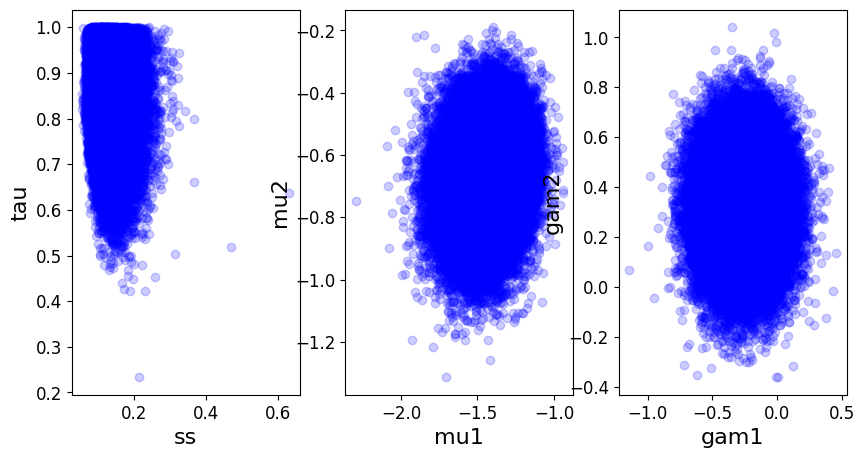
\includegraphics[width=.8\linewidth]{"./gibbs_dist.png"}
  \caption{\label{fig:mh_dist} Bivariate distributions for samples drawn from Gibbs sampling}
\end{figure}

\begin{figure}[H]
  \centering
  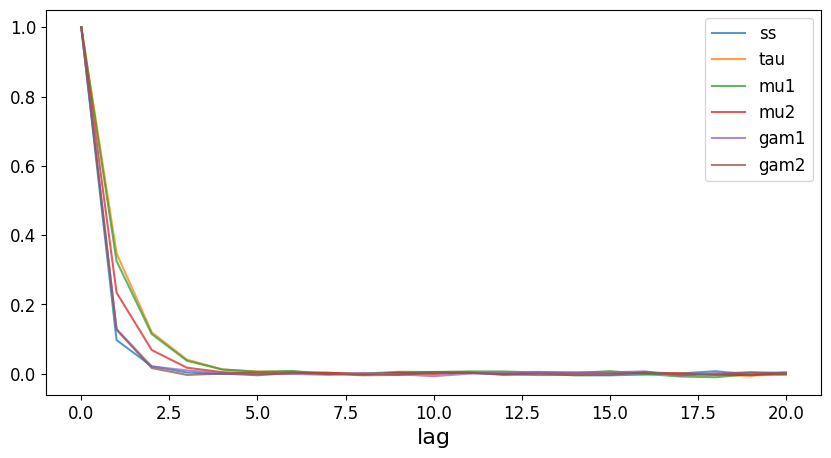
\includegraphics[width=.8\linewidth]{"./gibbs_acorr.png"}
  \caption{\label{fig:mh_acorr} Autocorrelation for each parameter value drawn from Gibbs sampling}
\end{figure}

\begin{figure}[H]
  \centering
  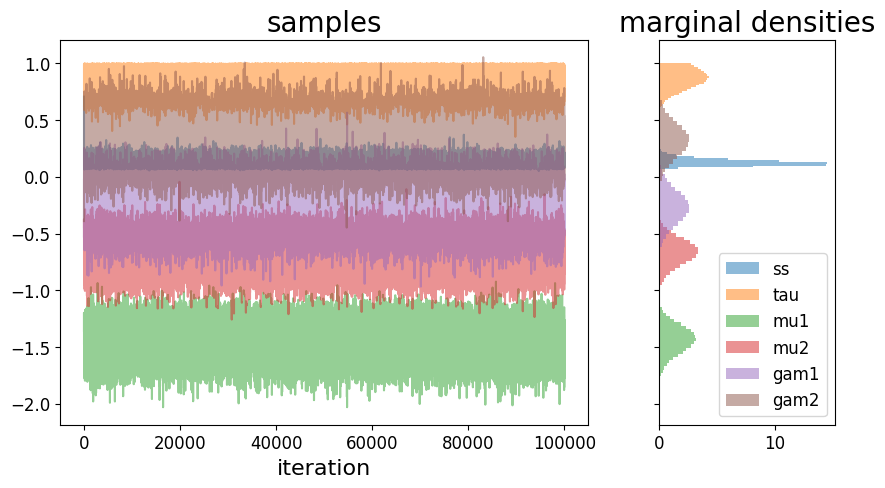
\includegraphics[width=.8\linewidth]{"./gibbs_marg.png"}
  \caption{\label{fig:mh_marg} Evolution of the Gibbs sampling algorithm and accumulated marginal distributions}
\end{figure}

Next I present univariate statistics in Table \ref{tab:gibbs_univar} as well as the covariance between each parameter pair in Table \ref{tab:gibbs_covar}. 

\begin{table}[H]
  \begin{center}
    \begin{tabular}{lrrrrrr}
      &$\sigma^2$ & $\tau$ & $\mu_1$ & $\mu_2$ & $\gamma_1$ & $\gamma_2$ \\
      \midrule
      mean   &  0.128855 &  0.856592 & -1.437832 & -0.660407 & -0.269792 &  0.316120 \\
      var    &  0.000854 &  0.007508 &  0.016422 &  0.013851 &  0.024934 &  0.023575 \\
      median &  0.124435 &  0.864481 & -1.432695 & -0.657491 & -0.270956 &  0.317396 \\
      p0     &  0.060584 &  0.389299 & -2.154638 & -1.326388 & -0.958255 & -0.361611 \\
      p10    &  0.095844 &  0.738386 & -1.602141 & -0.809834 & -0.470537 &  0.121178 \\
      p25    &  0.107768 &  0.798937 & -1.520030 & -0.735483 & -0.373689 &  0.214412 \\
      p50    &  0.124435 &  0.864481 & -1.432695 & -0.657491 & -0.270956 &  0.317396 \\
      p75    &  0.145736 &  0.924773 & -1.350404 & -0.580824 & -0.166230 &  0.418696 \\
      p90    &  0.167346 &  0.966222 & -1.279685 & -0.514553 & -0.070925 &  0.509682 \\
      p100   &  0.327578 &  0.999997 & -0.861472 & -0.172091 &  0.399618 &  0.980294 \\
      \bottomrule
      \end{tabular}
  \end{center}
  \caption{\label{tab:gibbs_univar} Univariate statistics from samples drawn from Gibbs sampling}
\end{table}

\begin{table}[H]
  \begin{center}
    \begin{tabular}{lrrrrrr}
      {} & $\sigma^2$ & $\tau$ & $\mu_1$ & $\mu_2$ & $\gamma_1$ & $\gamma_2$ \\
      \midrule
      $\sigma^2$   &  0.000829 & -0.000252 & -0.000165 & -0.000096 & -0.000002 & -0.000044 \\
      $\tau$  & -0.000252 &  0.007479 &  0.005188 &  0.003529 & -0.000656 &  0.000722 \\
      $\mu_1$  & -0.000165 &  0.005188 &  0.016047 &  0.002465 & -0.006474 &  0.000578 \\
      $\mu_2$  & -0.000096 &  0.003529 &  0.002465 &  0.014061 & -0.000331 & -0.005675 \\
      $\gamma_1$ & -0.000002 & -0.000656 & -0.006474 & -0.000331 &  0.023364 & -0.000024 \\
      $\mu_2$ & -0.000044 &  0.000722 &  0.000578 & -0.005675 & -0.000024 &  0.023471 \\
      \bottomrule
      \end{tabular}
  \end{center}
  \caption{\label{tab:gibbs_covar} Covariance between parameters from distributions drawn from Gibbs sampling}
\end{table}


% =================================== TODO ====================================
In these tables I observe PLACEHOLDER




% -------------------------------------------------------------------------------
% HMC
\section{Hamiltonian Monte Carlo}
\subsection*{Implementation}
\begin{itemize}
  \item Boundary constraints using Rollback HMC: https://arxiv.org/pdf/1709.02855.pdf and Reflection HMC: https://people.cs.umass.edu/~domke/papers/2015nips1.pdf
\end{itemize}

\begin{align*}
  H(q, p) =& U(q) + K(p) \textrm{, Hamiltonian function}\\
  & \textrm{with $U(\cdot)$, potential energy, $K(\cdot)$, kinetic energy, $q \in \mathbb{R}^k$, position, $p \in \mathbb{R}^k$ momentum}\\
  & \textrm{let } U(\theta) := -\log f(\theta) \textrm{, where } p(\theta | Y) = \frac{1}{C}f(\theta) \textrm{, and } p \sim N(0, \textbf{M})
\end{align*}

\subsection*{Results}


% -------------------------------------------------------------------------------
% IMPORTANCE SAMPLING
\section{Importance sampling}
\subsection{Implementation}
In this section I implement importance sampling with normalization to estimate sample statistics from my posterior distribution of model parameters. This technique allows me to draw samples, $\theta_i$, from a trial distribution, $q(\theta)$, and weight those samples with weights $u_i$ to achieve these sample statistics. Normalization allows me to use this approach for a function proportional to my target distribution, $f(\theta)$, up to an integrating constant (i.e., $p(\theta \mid Y) \propto\; f(\theta))$.

We show in class that importance sampling with normalization yields weighted samples where the sum of those weighted samples is a biased estimate of the expectation of the target distribution. Further, we have shown that the sum of any function of those weighted samples is a biased estimates of the expectation of that function, under the garget distribution.

\begin{align}
  \sum_i^n\theta_i w_i &\approxeq E\left[ \theta\right]\\
  \sum_i^nh(\theta_i)w_i &\approxeq E\left[ h(\theta) \right]
\end{align}

Like Metropolis-Hasting, implementing this method requires selecting a target distribution. A naive approach to this involves selecting a multivariate t-distribution with support covering that of the target distribution. The t-distribution with a low degree of freedom is a good choice for such a candidate because of its wider tails, allowing samples to be drawn with higher likelihood over a wider range. 

In this instance, however, I notice that I can implement a form of two-stage Importance Sampling where I can construct a candidate distribution closer to my target distribution. This is desireable because drawing samples closer to my target distribution can increase the efficiency of my algorithm.

I observe that my target distribution can be re-written as the outcome of sequential posterior distribution calculations. Specifically
\begin{align}
  p(\theta \mid Y) = p(\sigma^2, \tau, \mu, \gamma \mid Y) &\propto\; p(\sigma^2) p(\tau) p(\mu) p(\gamma)\times \prod_{i\in g_1, g_2, g_3, g_4} L(y_i \mid \sigma^2, \tau, \mu, \gamma)\\
  &\propto\; (\sigma^2) p(\mu) p(\gamma) \times \prod_{i\in g_1, g_2} L(y_i \mid \sigma^2, \mu, \gamma) \times p(\tau) \times \prod_{i\in g_3, g_4} L(y_i \mid \sigma^2, \tau, \mu, \gamma)\\
  &\propto\; p(\sigma^2, \mu, \gamma \mid Y_{1,2}) \times p(\tau) \times \prod_{i\in g_3, g_4} L(y_i \mid \sigma^2, \tau, \mu, \gamma)
\end{align}
I next observe that the posterior, $p(\sigma^2, \mu, \gamma \mid Y_{1,2})$ can be computed in closed form.
\begin{align}
  q(\sigma^2, \mu, \gamma \mid Y_{1,2}) &= q(\mu, \gamma \mid Y_{1,2}) \times q(\sigma^2 \mid \mu, \gamma, Y_{1,2}) \textrm{, where}\\
  q(\mu, \gamma \mid Y_{1,2}) &\sim t_4\left(\mu= \left(\begin{matrix*}
    \overline{Y_1}\\ \overline{Y_2} \end{matrix*}\right), \Sigma=\frac{\sum_{i\in g_1}\lVert y_i - \overline{Y_1} \rVert^2 + \sum_{i \in g_2}\lVert y_i - \overline{Y_2}\rVert^2}{\nu}\left(\begin{matrix*}
      n_1^{-1} & 0 & 0 & 0 \\ 0 & n_1^{-1} & 0 & 0 \\ 0 & 0 & n_2^{-1} & 0 \\ 0 & 0 & 0 & n_2^{-1}
    \end{matrix*}\right), \nu=2(n_1 + n_2) - 4\right)\\
  q(\sigma^2 \mid \mu, \gamma, Y_{1,2}) &\sim InvGamma\left(\alpha=n_1 + n_2, \beta = \frac{1}{2}\sum_{i\in g_1}\lVert y_i - \mu\rVert^2 + \sum_{i\in g_2}\lVert y_i - \gamma\rVert^2\right)
\end{align}
Lastly, I note that for a trial density $q(\theta) := p(\sigma^2, \mu, \gamma \mid Y_{1,2}) \times p(\tau)$, I can estimate unnormalized sample weights in a straightforward manner. Notably
\begin{align}
  w_i := \frac{p(\theta_i)}{q(\theta_i)} = \frac{p(\sigma^2, \tau, \mu, \gamma \mid Y)}{p(\sigma^2, \mu, \gamma \mid Y_{1,2}) \times p(\tau)} \propto\; \frac{p(\sigma^2, \mu, \gamma \mid Y_{1,2}) \times p(\tau) \times \prod_{i\in g_3, g_4} L(y_i \mid \sigma^2, \tau, \mu, \gamma)}{p(\sigma^2, \mu, \gamma \mid Y_{1,2})\times p(\tau)} = \prod_{i\in g_3, g_4} L(y_i \mid \sigma^2, \tau, \mu, \gamma) =: u_i
\end{align}
Using the normalization method proved in class lecture, it follows cleanly that $w_i = u_i / \sum_{j=1}^nu_j$. I present all derivations of the distributions above in Appendix \ref{sec:a_is}.

My sampling method is therefore
\begin{algorithm}
\caption{Importance sampling}
  \begin{algorithmic}
    \State $\theta_0 \longleftarrow$  Initialize
    \For{t=1, \dots, T}
      \State $\theta_i[\mu, \gamma] \sim q(\mu, \gamma \mid Y_{1,2})$
      \State $\theta_i[\sigma^2] \sim q(\sigma^2 \mid \theta_i[\mu, \gamma], Y_{1,2})$
      \State $\theta_i[\tau] \sim p(\tau)$
      \State $u_i = f(\theta_i \mid Y) / q(\theta_i)$  \Comment{$f(\theta_i \mid Y) \propto p(\theta_i \mid Y)$}
    \EndFor
    \State $\textbf{w} = \textbf{u} / \sum_{j=1}^n u_j$ \Comment{$\textbf{u}$ is a vector of all $u_i$}
    \State $\hat{\boldsymbol{\theta}} = \boldsymbol{\theta}*\textbf{w}$ \Comment{element-wise product; $\boldsymbol{\theta}$ is a vector of all $\theta_i$} 
  \end{algorithmic}
\end{algorithm}
\subsection*{Design choices, tuning, and scalability}
\subsection*{Results}

\section{Discussion and conclusion}
PLACEHOLDER -- Compare methods
% =================================== TODO ====================================
PLACEHOLDER FOR SCALABILITY
* MH, gibbs, and IS are O(n) 
* gibbs and IS are fastest
* HMC is O(n*l)



%------------------------------------------------------------------------
% REFERENCES
{\small
\bibliographystyle{ieee}
\bibliography{egbib}
}

%------------------------------------------------------------------------
% Appendix
\section{Appendix}
\subsection{Derivation of the posterior, $p(\theta \mid Y)$}
\subsubsection{Provided models for gene expression}
\begin{align*}
  (y_i | g_i = 1) &\sim N(\mu, \sigma^2 I)\\
  (y_i | g_i = 2) &\sim N(\gamma, \sigma^2 I)\\
  (y_i | g_i = 3) &\sim N(\frac{1}{2}(\mu + \gamma), \sigma^2 I)\\
  (y_i | g_i = 4) &\sim N(\tau\mu + (1-\tau)\gamma, \sigma^2 I)
\end{align*}
\subsubsection{Provided priors for gene expression models}
\begin{align*}
  \theta &= (\sigma^2, \tau, \mu_1, \mu_2, \gamma_1, \gamma_2)\\
  p(\sigma^2) &\propto \frac{1}{\sigma^2}\\
  p(\tau) &\sim Unif[0, 1]\\
  p(\mu) &= p(\mu_1, \mu_2) \propto 1 \textrm{ (improper uniform)}\\
  p(\gamma) &= p(\gamma_1, \gamma_2) \propto 1 \textrm{ (improper uniform)}\\
\end{align*}
\subsubsection{Derivation of likelihood and posterior distribution}
\begin{align*}
  L(Y | \theta) =& \prod_{i=1}^n p(y_i | \theta) \textrm{, for } Y = (y_i, \dots, y_n)\\
  =& \prod_{i \in g_1} \frac{1}{\sqrt{2\pi}}((\sigma^2)^2)^{-\frac{1}{2}} \exp[-\frac{1}{2\sigma^2} (y_i - \mu)^T(y_i - \mu)] \times  
     \prod_{i\in g_2} \frac{1}{\sqrt{2\pi}}((\sigma^2)^2)^{-\frac{1}{2}} \exp[-\frac{1}{2\sigma^2} (y_i - \gamma)^T(y_i - \gamma)]\\
  &\times \prod_{i\in g_3} \frac{1}{\sqrt{2\pi}}((\sigma^2)^2)^{-\frac{1}{2}} \exp[-\frac{1}{2\sigma^2} (y_i - \frac{1}{2}(\mu +  
    \gamma))^T(y_i - \frac{1}{2}(\mu + \gamma))] \\
  &\times \prod_{i\in g_4} \frac{1}{\sqrt{2\pi}}((\sigma^2)^2)^{-\frac{1}{2}} \exp[-\frac{1}{2\sigma^2} (y_i - (\tau\mu + (1-\tau)\gamma))^T(y_i - (\tau\mu + (1-\tau)\gamma))] \\
  =& \left(\frac{1}{\sigma^2\sqrt{2\pi}}\right)^n \exp[-\frac{1}{2\sigma^2}(\sum_{i\in g_1}(y_i - \mu)^T(y_i -   \mu) + \sum_{i\in g_2}(y_i - \gamma)^T(y_i - \gamma)\\
  &+ \sum_{i\in g_3}(y_i - \frac{1}{2}(\mu +  
  \gamma))^T(y_i - \frac{1}{2}(\mu + \gamma)) + \sum_{i\in g_4}(y_i - (\tau\mu + (1-\tau)\gamma))^T(y_i - (\tau\mu + (1-\tau)\gamma)))]\\\\
  p(\theta | Y) \propto&\; p(\theta) L(Y | \theta)
\end{align*}

\subsection{Metropolis Hasting}
\label{sec:a_mh}
\subsubsection{Results of hyperparameter tuning}
\begin{table}
  \begin{center}
\begin{tabular}{lllrr}
  $\nu_{\sigma^2}$ & $\nu_\tau$ & $\nu_{\mu, \gamma}$ & \textbf{Acceptance rate} & \textbf{Max lag $\leq 0.2$} \\
  \midrule
  0.005 &    0.01 &   0.01 &         0.311667 &           94.0 \\
  0.001 &    0.01 &   0.01 &         0.373333 &           84.0 \\
  0.050 &    0.01 &   0.01 &         0.253333 &           36.0 \\
  0.005 &    0.05 &   0.01 &         0.206667 &           79.0 \\
  0.001 &    0.05 &   0.01 &         0.248333 &           63.0 \\
  0.050 &    0.05 &   0.01 &         0.198333 &           44.0 \\
  0.005 &    0.10 &   0.01 &         0.193333 &          153.0 \\
  0.001 &    0.10 &   0.01 &         0.233333 &           85.0 \\
  0.050 &    0.10 &   0.01 &         0.171667 &           32.0 \\
  0.005 &    0.01 &   0.05 &         0.091667 &           65.0 \\
  0.001 &    0.01 &   0.05 &         0.165000 &          142.0 \\
  0.050 &    0.01 &   0.05 &         0.110000 &           32.0 \\
  0.005 &    0.05 &   0.05 &         0.088333 &          157.0 \\
  0.001 &    0.05 &   0.05 &         0.128333 &          149.0 \\
  0.050 &    0.05 &   0.05 &         0.066667 &           43.0 \\
  0.005 &    0.10 &   0.05 &         0.040000 &           89.0 \\
  0.001 &    0.10 &   0.05 &         0.123333 &          176.0 \\
  0.050 &    0.10 &   0.05 &         0.055000 &           73.0 \\
  0.005 &    0.01 &   0.10 &         0.031667 &           68.0 \\
  0.001 &    0.01 &   0.10 &         0.045000 &          111.0 \\
  0.050 &    0.01 &   0.10 &         0.045000 &           42.0 \\
  0.005 &    0.05 &   0.10 &         0.066667 &          165.0 \\
  0.001 &    0.05 &   0.10 &         0.065000 &           60.0 \\
  0.050 &    0.05 &   0.10 &         0.026667 &          136.0 \\
  0.005 &    0.10 &   0.10 &         0.051667 &          156.0 \\
  0.001 &    0.10 &   0.10 &         0.078333 &          176.0 \\
  0.050 &    0.10 &   0.10 &         0.023333 &           74.0 \\
 \bottomrule
 \end{tabular}
\end{center}
 \caption{\label{tab:mh_gridsearch} Grid search across candidate distribution variances}
\end{table}


\subsection{Gibbs sampling}
\label{sec:a_gibbs}
\subsubsection{Derivation of $p(\tau \mid \sigma^2, \mu, \gamma, Y)$}
\begin{align*}
  p(\tau | Y, \theta[-\tau]) &\propto p(\theta)L(Y | \theta)\\  
  & \propto p(\tau)\prod_{i\in g_4} \frac{1}{\sigma^2\sqrt{2\pi}} \exp[-\frac{1}{2\sigma^2} (y_i - (\tau\mu + (1-\tau)\gamma))^T(y_i - (\tau\mu + (1-\tau)\gamma))]\\
  &\propto \exp[-\frac{1}{2\sigma^2}\sum_{i\in g_4}(y_i - (\tau\mu + (1-\tau)\gamma))^T(y_i - (\tau\mu + (1-\tau)\gamma))] \textrm{, for } \tau \in [0,1]\\
  &\propto \exp[-\frac{1}{2\sigma^2}\sum_{i\in g_4}(y_i^Ty_i - 2y_i^T(\tau\mu + (1-\tau)\gamma) + (\tau\mu + (1-\tau)\gamma)^T(\tau\mu + (1-\tau)\gamma))] \textrm{, for } \tau \in [0,1]\\
  &\propto \exp[-\frac{1}{2\sigma^2}\sum_{i\in g_4} \tau^2(\mu^T\mu - 2\mu^T\gamma + \gamma^T\gamma) - 2\tau(y_i^T\mu - y_i^T\gamma - \mu^T\gamma + \gamma^T\gamma)]\textrm{, for } \tau \in [0,1]\\
  &\propto \exp[-\frac{1}{2\sigma^2}(n_4 \tau^2(\mu - \gamma)^T(\mu - \gamma) - 2\tau(\mu - \gamma)^T[\sum_{i\in g_4}(y_i - \gamma) \textrm{, for } \tau \in [0,1]\\
  &\propto \exp\left[-\frac{1}{2}*\frac{n_4(\mu - \gamma)^T(\mu - \gamma)}{\sigma^2}\left(\tau - \frac{(\mu - \gamma)^T(\sum_{i\in g_4}(y_i - \gamma))}{n_4(\mu - \gamma)^T(\mu - \gamma)}\right)^2\right] \textrm{, for } \tau \in [0,1]\\
  &\sim Norm\left(\mu=\frac{(\mu - \gamma)^T(\sum_{i\in g_4}(y_i - \gamma))}{n_4(\mu - \gamma)^T(\mu - \gamma)}, \sigma^2=\frac{\sigma^2}{n_4(\mu - \gamma)^T(\mu - \gamma)}\right) \textrm{, truncated to } [0,1]
\end{align*}

\subsubsection*{Derivation of $p(\sigma^2 \mid \tau, \mu, \gamma, Y)$}
\begin{align*}
  p(\sigma^2 \mid Y, \theta[-\sigma^2]) \propto& p(\theta)L(Y | \theta) \propto p(\sigma^2) \prod_{i=1}^n p(y_i | \theta)\\
  \propto& \frac{1}{\sigma^2} * \left(\frac{1}{\sigma^2}\right)^n \exp\left[-\frac{1}{2\sigma^2}M\right] \textrm{, where } M = \\
  &\;\;\; \sum_{i\in g_1}(y_i - \mu)^T(y_i -   \mu) + \sum_{i\in g_2}(y_i - \gamma)^T(y_i - \gamma)+ \sum_{i\in g_3}(y_i - \frac{1}{2}(\mu +  
  \gamma))^T(y_i - \frac{1}{2}(\mu + \gamma))\\
  &\;\;\; + \sum_{i\in g_4}(y_i - (\tau\mu + (1-\tau)\gamma))^T(y_i - (\tau\mu + (1-\tau)\gamma))\\
  \propto& (\sigma^2)^{-n - 1}\exp\left[-\frac{M}{2}\frac{1}{\sigma^2}\right]\\
  \sim& InvGamma\left(\alpha=n, \beta = \frac{M}{2}\right)
\end{align*}

\subsubsection{Derivation of $p(\mu \mid \sigma^2, \tau, \gamma, Y)$}
\begin{align*}
  p(\mu | Y, \theta[-\mu]) \propto& p(\theta)L(Y | \theta)\\
  \propto& \prod_{i \in g_1} \frac{1}{\sigma^2\sqrt{2\pi}} \exp[-\frac{1}{2\sigma^2} (y_i - \mu)^T(y_i - \mu)]
    \times \prod_{i\in g_3} \frac{1}{\sigma^2\sqrt{2\pi}} \exp[-\frac{1}{2\sigma^2} (y_i - \frac{1}{2}(\mu +  
    \gamma))^T(y_i - \frac{1}{2}(\mu + \gamma))] \\
  &\times \prod_{i\in g_4} \frac{1}{\sigma^2\sqrt{2\pi}} \exp[-\frac{1}{2\sigma^2} (y_i - (\tau\mu + (1-\tau)\gamma))^T(y_i - (\tau\mu + (1-\tau)\gamma))]\\
  \propto& \exp[-\frac{1}{2\sigma^2}(n_1\mu^T\mu - 2\mu^T\left(\sum_{i\in g_1}y_i\right) - \mu^T\left(\sum_{i\in g_3}y_i\right) + \frac{n_3}{4}\mu^T\mu + \frac{n_3}{2}\mu^T\gamma\\
  &-2\tau\mu^T\left(\sum_{i\in g_4}y_i\right) + \tau^2n_4\mu^T\mu + 2\tau(1 - \tau)n_4\mu^T\gamma )]\\
  \propto& \exp\left[-\frac{1}{2\sigma^2}(n_1 + \frac{n_3}{4} + n_4\tau^2)\left(\mu^T\mu - 2\mu^T\frac{\sum_{i \in g_1}y_i + \frac{1}{2}\sum_{i\in g_3}y_i + \tau\sum_{i\in g_4}y_i - (\frac{n_3}{4} + n_4\tau(1 - \tau))\gamma}{n_1 + \frac{n_3}{4} + n_4\tau^2} \right)\right] \\
  \propto& \exp\left[-\frac{1}{2\phi^2}(\mu - \psi)^T(\mu - \psi)\right] \textrm{, where }\\
  &\;\;\; \psi = \frac{\sum_{i \in g_1}y_i + \frac{1}{2}\sum_{i\in g_3}y_i + \tau\sum_{i\in g_4}y_i - (\frac{n_3}{4} + n_4\tau(1 - \tau))\gamma}{n_1 + \frac{n_3}{4} + n_4\tau^2} \textrm{, } \phi^2 = \frac{\sigma^2}{n_1 + \frac{n_3}{4} + n_4\tau^2}\\
  \sim& N(\mu = \psi, \Sigma = \phi^2 I)
\end{align*}

\subsubsection{Derivation of $p(\gamma \mid \sigma^2, \tau, \mu, Y)$}
By symmetry with posterior conditional probability of $\mu$,
\begin{align*}
  p(\gamma | Y, \theta[-\gamma]) \sim& N(\mu = \psi', \Sigma = \phi'^2 I) \textrm{, where }\\
  &\;\;\; \psi' = \frac{\sum_{i \in g_2}y_i + \frac{1}{2}\sum_{i\in g_3}y_i + (1-\tau)\sum_{i\in g_4}y_i - (\frac{n_3}{4} + n_4\tau(1 - \tau))\mu}{n_2 + \frac{n_3}{4} + n_4(1-\tau)^2} \textrm{, } \phi'^2 = \frac{\sigma^2}{n_2 + \frac{n_3}{4} + n_4(1-\tau)^2}
\end{align*}

\subsection{Importance sampling}
\label{sec:a_is}
\subsubsection{Derivation of $p(\sigma^2 \mid \mu, \gamma, Y_{1,2})$}
\begin{align*}
  q(\sigma^2 \mid \mu, \gamma, Y_{1,2})\propto&\;\; \frac{1}{\sigma^2} * \left(\frac{1}{\sigma^2}\right)^{n_1 + n_2} \exp\left[-\frac{1}{2\sigma^2}M\right] \textrm{, where } M = \sum_{i\in g_1}(y_i - \mu)^T(y_i -   \mu) + \sum_{i\in g_2}(y_i - \gamma)^T(y_i - \gamma)\\
  \propto&\;\; (\sigma^2)^{-n_1 - n_2 - 1}\exp\left[-\frac{M}{2}\frac{1}{\sigma^2}\right]\\
  \sim& InvGamma\left(\alpha=n_1 + n_2, \beta = \frac{M}{2}\right)
\end{align*}

\subsubsection{Derivation of $p(\mu, \gamma \mid Y_{1,2})$}
\begin{align*}
  q(\mu, \gamma \mid Y_{1,2}) =& \int_0^\infty q(\mu, \gamma, \sigma^2 \mid Y_{1,2})d\sigma^2\\
  \propto&\; \int_0^\infty\left(\frac{1}{\sigma^2}\right)^{n_1 + n_2 + n_3 + 1} \exp\left[-\frac{1}{2\sigma^2}(\sum_{i\in g_1} \lVert y_i - \mu\rVert^2 + \sum_{i\in g_2}\lVert y_i - \gamma \rVert^2\right]d\sigma^2\\
  \propto&\; \Gamma(n_1 + n_2) \left(-\frac{1}{2}  \sum_{i\in g_1} \lVert y_i - \mu\rVert^2 + \sum_{i\in g_2}\lVert y_i - \gamma \rVert^2\right)^{-(n_1 + n_2)}, \textrm{ where } \frac{\Gamma(\alpha)}{\beta^\alpha} = \int_0^\infty (\sigma^2)^{-\alpha - 1} \exp\left(\frac{\beta}{\sigma^2}\right)d\sigma^2\\
  \propto&\; (M + n_1\lVert \overline{Y_1} - \mu \rVert^2 + n_2\lVert \overline{Y_2} - \gamma \rVert^2)^{-(n_1 + n_2)}, \textrm{ where } M = \sum_{i\in g_1}\lVert y_i - \overline{Y_1} \rVert^2 + \sum_{i\in g_2}\lVert y_i - \overline{Y_2} \rVert^2\\
  \propto&\; \left(M + \left[\left(\begin{matrix}\mu\\ \gamma\end{matrix}\right) - \left(\begin{matrix*}\overline{Y_1}\\ \overline{Y_2}\end{matrix*}\right)\right]^T \left(\begin{matrix*} n_1 & 0 & 0 & 0 \\ 0 & n_1 & 0 & 0 \\ 0 & 0 & n_2 & 0 \\ 0 & 0 & 0 & n_2 \end{matrix*}\right) \left[\left(\begin{matrix}\mu\\ \gamma\end{matrix}\right) - \left(\begin{matrix*}\overline{Y_1}\\ \overline{Y_2}\end{matrix*}\right)\right]\right)^{-(n_1 + n_2)}\\
  \propto&\; \left(1 + \frac{1}{2(n_1 + n_2) - 4}\times\frac{2(n_1 + n_2) - 4}{M}\left[\left(\begin{matrix}\mu\\ \gamma\end{matrix}\right) - \left(\begin{matrix*}\overline{Y_1}\\ \overline{Y_2}\end{matrix*}\right)\right]^T \left(\begin{matrix*} n_1^{-1} & 0 & 0 & 0 \\ 0 & n_1^{-1} & 0 & 0 \\ 0 & 0 & n_2^{-1} & 0 \\ 0 & 0 & 0 & n_2^{-1} \end{matrix*}\right)^{-1} \left[\left(\begin{matrix}\mu\\ \gamma\end{matrix}\right) - \left(\begin{matrix*}\overline{Y_1}\\ \overline{Y_2}\end{matrix*}\right)\right]\right)^{-(n_1 + n_2)}\\
  \propto&\; \left[1 + \frac{1}{\nu}(x - \eta)^T\Sigma^{-1}(x - \eta)\right]^{-\frac{\nu + 4}{2}}, \textrm{where }\\
  &\;\; \nu=2(n_1 + n_2) + 4, \Sigma=\frac{M}{2(n_1 + n_2) - 4}\left(\begin{matrix*} n_1^{-1} & 0 & 0 & 0 \\ 0 & n_1^{-1} & 0 & 0 \\ 0 & 0 & n_2^{-1} & 0 \\ 0 & 0 & 0 & n_2^{-1} \end{matrix*}\right), \eta=\left(\begin{matrix*}\overline{Y_1}\\ \overline{Y_2}\end{matrix*}\right)\\
  q(\mu, \gamma \mid Y_{1,2}) &\sim t_4\left(\mu= \left(\begin{matrix*}
    \overline{Y_1}\\ \overline{Y_2} \end{matrix*}\right), \Sigma=\frac{\sum_{i\in g_1}\lVert y_i - \overline{Y_1} \rVert^2 + \sum_{i \in g_2}\lVert y_i - \overline{Y_2}\rVert^2}{\nu}\left(\begin{matrix*}
      n_1^{-1} & 0 & 0 & 0 \\ 0 & n_1^{-1} & 0 & 0 \\ 0 & 0 & n_2^{-1} & 0 \\ 0 & 0 & 0 & n_2^{-1}
    \end{matrix*}\right), \nu=2(n_1 + n_2) - 4 \right)
\end{align*}
\end{document}
